Welche Typen von Beziehungen gibt es zwischen Klassen und wie werden sie in der UML dargestellt?


\section*{Antwort}

\begin{figure}
    \centering
    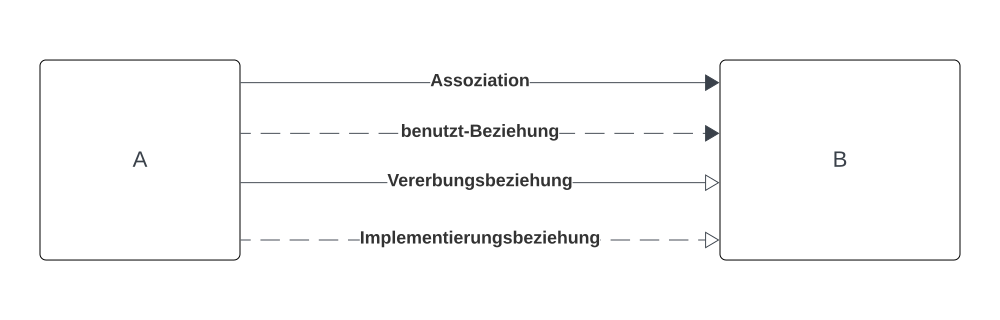
\includegraphics[scale=0.4]{chapters/aufgabe 1/img/umldependencies}
    \caption{Verschiedene Ausprägungen von Abhängigkeitsbeziehungen zwischen Klassen.
    Zusätzlich aufgeführt ist die \textit{Implementierungsbeziehung},die eine Beziehung zwischen einer \textit{Schnittstelle} und einer \textit{Klasse} darstellt (Quelle: eigene)}
    \label{fig:umldependencies}
\end{figure}

\begin{itemize}
    \item \textbf{Abhängigkeiten} - gestrichelte Linie, Pfeilspitze Richtung der Klasse, zu der eine Abhängigkeit besteht (s. auch ``benutzt-Beziehung`` in Abbildung~\ref{fig:umldependencies})
    \item \textbf{Assoziationen} - durchgezogene Linie, optional Kardinalitäten an den beiden Enden einer Linie.
    Optionale Pfeile geben die \textbf{Navigierbarkeit} an.
    Werden \textit{keine} Pfeile oder Pfeile \textit{jeweils} an Quell-/Zielklasse angegeben, ist die Assoziation \textit{bidirektional}\footnote{
    ``An association with neither end marked by navigability arrows means that the association is navigable in both
    directions.`` (\cite[18]{UML17})
    }, ansonsten unidirektional: Eine Klasse kann dann die Assoziation in Richtung Pfeilspitze abfragen
    \item \textbf{Vererbungsbeziehungen}: durchgezogene Linie, abgeschlossene, nicht gefüllte Pfeilspitze (``Dreieck``) in Richtung der Basisklasse, ausgehend von der spezialisierten Klasse (vgl.~\cite[52]{Bal05})
\end{itemize}